\section{Introduction}
Geometric range searching is one of the most common types of 
problems which arise in several applications. Here, a set of 
geometric objects $S$ are given, such as points, lines, circles, 
or boxes, and the query is with respect to another well-defined 
geometric object $Q$ where the objective is to identify all 
elements in $S$ contained within the query region $Q$. 
Traditionally, preprocessing scheme is developed to build a data 
structure so that it can answer the query as efficiently as 
possible. Depending on the complexity of the objects in $S$, the 
query region $Q$ and the query requirement, a great deal of 
research was done in this area.  

In this paper, we address the notion of \emph{partial enclosure range searching (\PERS{})}, which, to the best of our knowledge, has not been explored previously. 
In this setting, our goal is to identify, for a given query region, all objects which satisfy the \emph{partial enclosure property}, which specifies that an object must intersect a query region by at least some fixed proportion of the object's own size (e.g., length, area, volume) in order to be selected.

This problem was inspired by the use of Microsoft OneNote. 
Using a digital pen, OneNote can be used much like a paper notebook, allowing the user to add handwriting, diagrams, equations, and any other such thing to a page.
Unlike a paper notebook, OneNote also allows the user to select previously drawn objects in order to translate, scale, copy and otherwise manipulate them.
Figure~\ref{fig:intro:onenote} shows some handwritten notes, and a diagram which has been partially selected.

\begin{figure}[t]
\begin{center}
  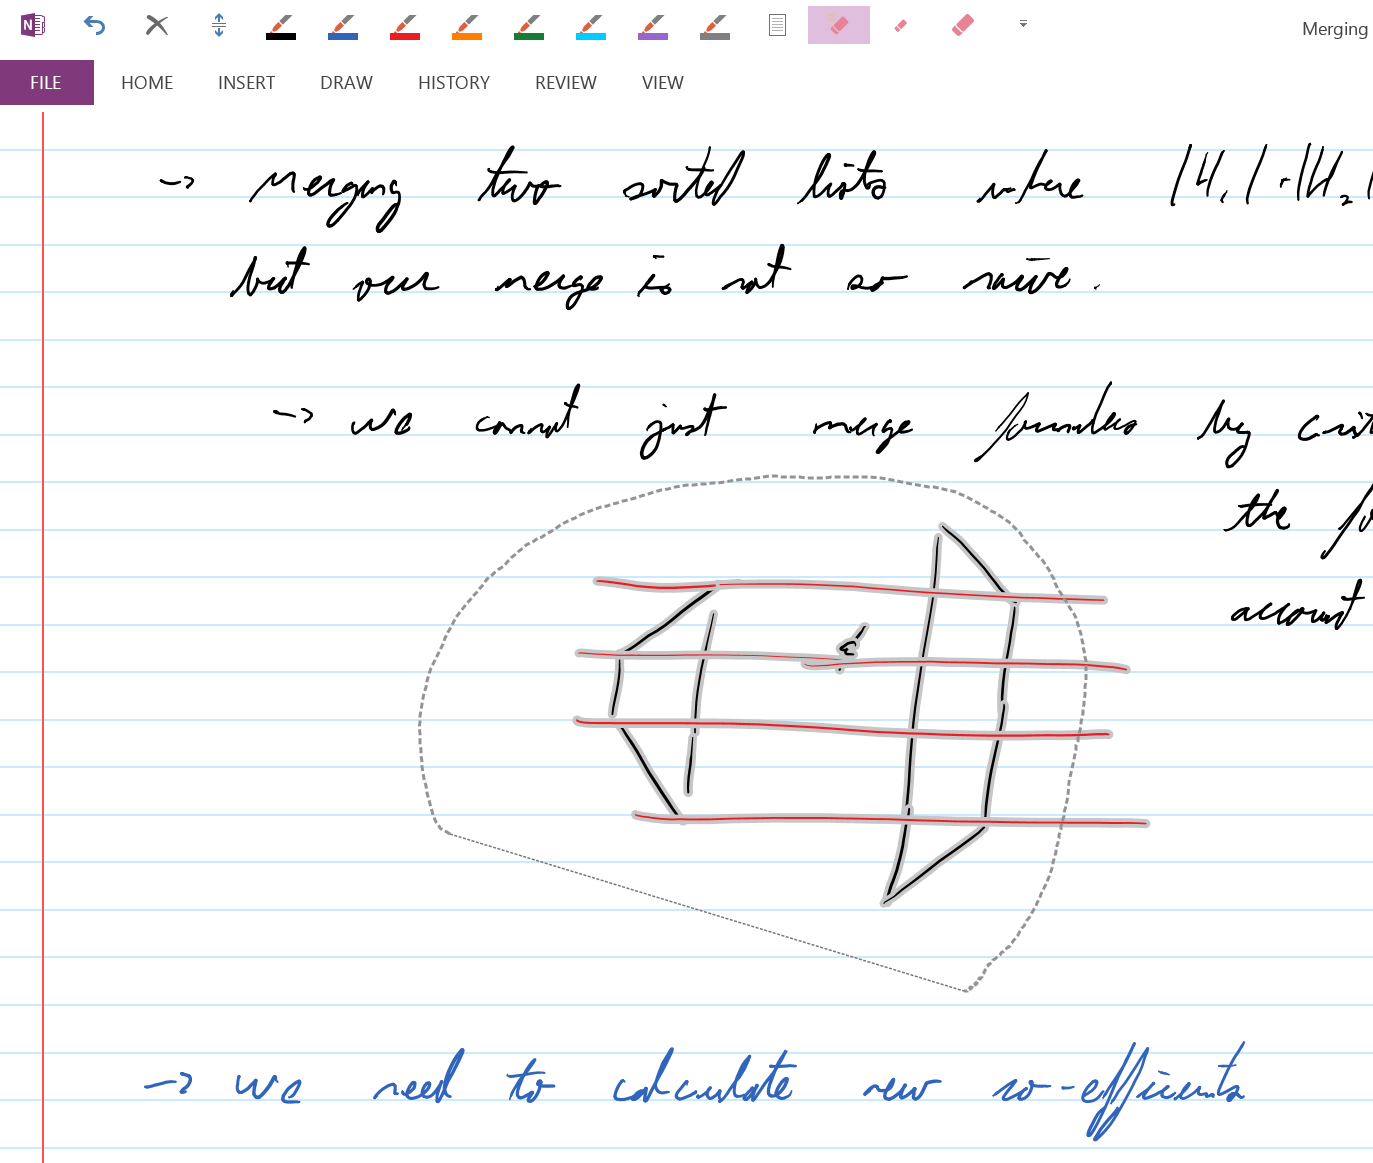
\includegraphics[width=0.50\textwidth]{figures/fig_onenote}
  \caption[An example of practical partial enclosure range searching]{An example of practical partial enclosure range searching in Microsoft OneNote. The line segments in the middle are selected even though they are not entirely enclosed in the query region.}
  \label{fig:intro:onenote}
\end{center}
\end{figure}

Looking carefully at the figure, we can see that even though the horizontal line segments of the diagram have not been entirely enclosed by the selection tool, they nevertheless appear as part of the set of selected items.
This behaviour of selecting partially enclosed objects is described in a patent filed by Microsoft Corporation \cite{lassoselect}. 
From the patent:

\begin{quote}
[T]here is a need for a selection tool that will allow a user to conveniently select one or more graphical objects in their entirety, without requiring an inconvenient amount of precision from the user.
\end{quote}

\noindent With the rising popularity of touch and pen-enabled devices, this need is likely to increase.  
Although the problems that we will examine take place in simpler settings, we will nevertheless develop an understanding of the major challenges of this problem domain, as well as some techniques for addressing them.



The paper proposes algorithms for the following partial enclosure range search settings.  
\begin{description}
\item[Partial enclosure range searching:] Here $S$ is a given a set of line segments, 
and the query object $Q$ is with respect to a rectangle or a slab bounded by two parallel lines. The objective is to report/count the number of objects in $S$ that lie in $Q$. We have considered different combinations depending on the orientation of the 
line segments in $S$ and the orientation of the rectangle/slab $Q$.
\item[Partial enclosure volume computation:] Here $S$ is a given convex/monotone/arbitrary polygon, and $Q$ is an axis-parallel rectangle/slab. The objective is to compute the area of the region $S\cap Q$. 
\end{description}

Table~\ref{tab:contributions} gives a broad overview of the proposed results in this paper. 
Here, `AP' is used for ``Axis-Parallel'', `AO' for ``Arbitrary Orientation'', `P' for ``Polygon''.

\begin{table}[t]
\caption{Summary of Contributions}
\label{tab:contributions}
\centering
\begin{tabular}{l l l l l l}
\hline \hline
Object & Query & Theorem & Space & Time & Query \\
\hline
AP Segment & AP Rectangle & Th~\ref{th:ap} & $O(n\log^3n)$ & $O(n\log^3n)$ & $O(\log^3n$ \\
AO Segment & AP Rectangle & Th~\ref{th:ao} & $O(n\log^7n)$ & $O(n\log^7n)$ & $O(\sqrt{n}\log^7n)$ \\
AP Segment & AO Slab & Th~\ref{th:slabs:one} & $O(n\log^2n)$ & $O(n\log^3n)$ & $O(\sqrt{n}\log^3n)$ \\
AP Segment & 2 AO Slabs & Th~\ref{th:slabs:two} & $O(n\log^3n)$ & $O(n\log^3n)$ & $O(\sqrt{n}\log^3n)$ \\
Convex P & Rectangle & Th~\ref{th:convexp:area} & $O(n)$ & $O(n)$ & $O(\log n)$ \\
Convex P & Convex $k$-gon & Cor~\ref{cor:convexp:karea} & $O(n)$ & $O(n)$ & $O(k \log n)$ \\
Monotone P & AP Rectangle & Th~\ref{th:monotonep:rect:area} & $O(n\log n)$ & $O(n\log n)$ & $O(\log n)$ \\
Monotone P & AP Rectangle & Th~\ref{th:mono2} & $O(n)$ & $O(n\log n)$ & $O(\sqrt{n})$ \\
Simple P & Horiz Slab & Cor~\ref{cor:monotonep:simplep-area} & $O(n)$ & $O(n)$ & $O(\log n)$ \\
\hline
\end{tabular}
\end{table}


The paper is organized as follows. Section  
~\ref{:prelim} reviews the useful data structures and range searching techniques which we utilize in our contributions.
The next four chapters cover partial enclosure range searching queries on successively more sophisticated geometric objects, with Sectionr~\ref{:rectangles} focusing on axis-parallel rectangles, Section~\ref{:slabs} on arbitrarily-oriented slabs, Section~\ref{:convexp} on convex polygons, and Section~\ref{:monotonep} on monotone polygons.
Finally, we conclude in Section~\ref{:conclusion}, where we summarize our contributions and future work. 
